\subsection*{Medical Transformer: Gated Axial-Attention for
Medical Image Segmentation}

% \subsection*{Ссылка} \url{https://arxiv.org/abs/2102.10662}
\subsubsection*{Введение}
Сверточные нейронные сети сравнительно плохо понимают зависимости между признаками, которые находятся на дальнем расстоянии друг от друга
в изображениях. Недавно предложенные архитекутры сетей, основанные на
трансформерах \cite{Transformers}, используют механизм самовнимания \cite{SelfAttention} для шифрования дальних
зависимостей и выявляют наиболее заметные представления. Эти наблюдения
мотивировали авторов статьи исследовать решения, в основе которых лежат
трансформеры и изучить возможность использования архитектур нейронных
сетей с трансформерами в задачах медицинской сегментации. \cite{MedT} 

\subsection*{Основная идея}
В данной работе предлагается закрытый, чувствительный к расположению axial 
attention механизм, который хорошо показывает себя на малых
наборах данных. Также, вводится эффективная методология обучения Local-
Global (LoGo) для трансформеров и Medical-Transformer (MedT) - метод,
построенный на основе двух вышеперечисленных предложенных концепций,
разработанный специально для сегментации медицинских изображений, который успешно улучшает производительность по сравнению со сверточными
нейронными сетями и сетями чисто attention архитектуры на трех разных датасетах. Предложенные методы
превосходят существующие в задаче сегментации медицинских изображений
не требуя при этом большого набора тренировочных данных. \\


Local-Global training:\\

Чтобы улучшить общее понимание изображения, предлагается использовать 
два ответвления сети - глобальная ветвь, которая работает с 
изображением оригинальной размерности и локальная ветвь для работы с патчами. 
В локальной ветви создается 16 патчей размера \(I/4 \times I/4\), каждый патч 
пропускается через сеть и выходные карты признаков resampled, основываясь на их расположении, 
чтобы получить итоговые карты признаков. К итоговым картам двух ветвей применяется 
свертка \(1\times 1\) и на выходе получается маска сегментации. 
Такая стратегия улучшает производительность, так как глобальная ветвь 
фокусируется на высокоуровневой информации, а локальная лучше определяет детали.

\begin{minipage}{1.0\linewidth}
    \begin{center}
        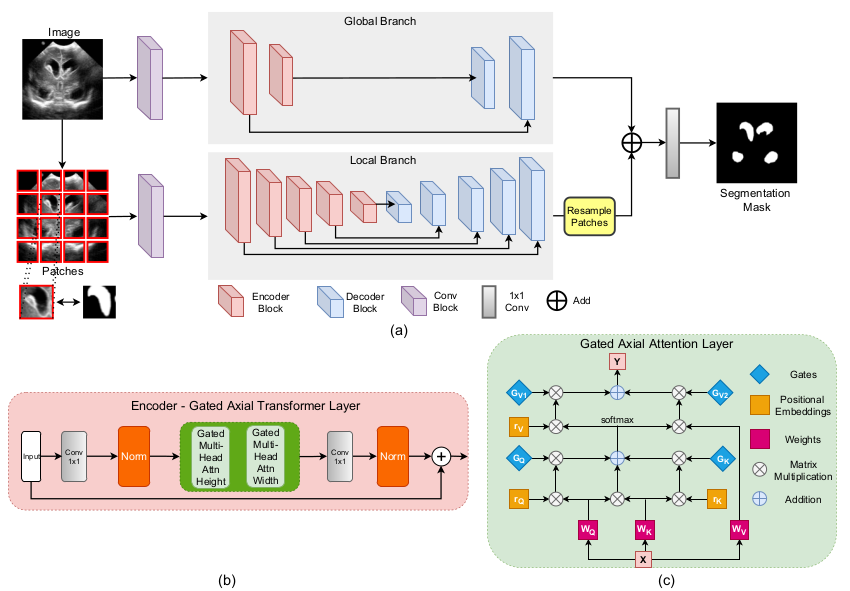
\includegraphics[scale=0.35]{ann18_arch.png} \\
        \captionof{figure}{\scriptsize{
           Архитектура MedT.
        }}
    \end{center}
    
\end{minipage} 
\subsection*{Данные}
Brain US, Glas, MoNuSeg
% \newpage
\subsection*{Результаты}
% \begin{minipage}{1.0\linewidth}
%     \begin{center}
%         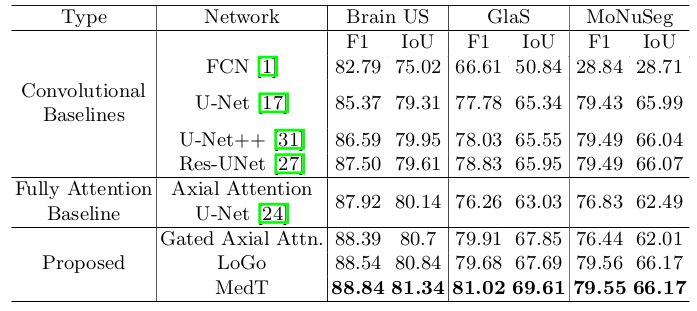
\includegraphics[scale=0.5]{ann18_res.png} \\
%         % \caption{\scriptsize{
%         %    Количественное сравнение предложенных методов со сверточными бейзлайнами, основанными на трансформерах
%         %    по мерам F1 и IoU.
%         % }}
%     \end{center}
    
% \end{minipage} 

{\small

\begin{center}
\captionof{table}{
       Количественное сравнение предложенных методов со сверточными бейзлайнами, основанными на трансформерах
       по мерам F1 и IoU.}
\begin{tabular}{
    |c | c | c  c | c c | c c |}
\hline
Type                                                               & Network                                                     & \multicolumn{2}{c|}{\cellcolor[HTML]{FFFFFF}Brain US} & \multicolumn{2}{c|}{\cellcolor[HTML]{FFFFFF}GlaS} & \multicolumn{2}{c|}{\cellcolor[HTML]{FFFFFF}MoNuSeg} \\ \hline
&                                                             & F1                         & IoU                        & F1                   & IoU                  & F1                    & IoU                   \\ \cline{3-8} 
& FCN                                                       & 82.79                           & 75.02                       & 66.61                     & 50.84                 & 28.84                      & 28.71                  \\
\begin{tabular}[c]{@{}c@{}}Convolutional \\ Baselines\end{tabular} & U-Net                                                      & 85.37                           & 79.31                       & 77.78                     & 65.34                 & 79.43                      & 65.99                  \\
& U-Net++                                                 & 86.59                           & 79.95                       & 78.03                          & 65.55                      & 79.49                           & 66.04                       \\
& Res-UNet                                                  & 87.50                            & 79.61                       & 78.83                     & 65.95                 & 79.49                      & 66.07                  \\ \hline
\begin{tabular}[c]{@{}c@{}}Fully Attention \\ Baseline\end{tabular}    & \begin{tabular}[c]{@{}c@{}}Axial Attention\\ U-Net\end{tabular} & 87.92                           & 80.14                       & 76.26                     & 63.03                 & 76.83                      & 62.49                  \\ \hline
& Gated Axial Attn.                                           & 88.39                           & 80.7                        & 79.91                     & 67.85                 & 76.44                      & 62.01                  \\
Proposed                                                           & LoGo                                                        & 88.54                           & 80.84                       & 79.68                     & 67.69                 & 79.56                      & 66.17                  \\
& MedT                                                        & \textbf{88.84}                           & \textbf{81.34}                       & \textbf{81.02}                     & \textbf{69.61}                 & \textbf{79.55}                      & \textbf{66.17}    \\ \hline             
\end{tabular}

    
\end{center}

}






% \begin{minipage}{1.0\linewidth}
%     \begin{center}
%         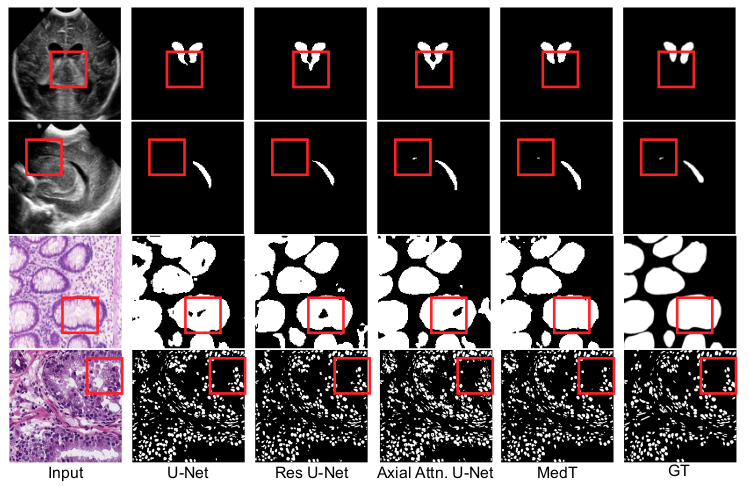
\includegraphics[scale=0.5]{ann18_mri.png} \\
%         \captionof{figure}{\scriptsize{
%             Качественные результаты на примерах тестовых изображений из датасетов Brain US, Glas и MoNuSeg.
%             Красный прямоугольник очерчивает регионы, где именно MedT показывает лучшие результаты, чем 
%             другие методы в сравнении.
%         }}
%     \end{center}
% \end{minipage}

\subsection*{Заключение}
В данной статье было продемонстрировано, что предложенные методы превосходят существующие 
в задаче сегментации медицинских изображений не требуя при этом большого набора тренировочных данных.





